\documentclass[8pt]{beamer}\usepackage[]{graphicx}\usepackage[]{color}
%% maxwidth is the original width if it is less than linewidth
%% otherwise use linewidth (to make sure the graphics do not exceed the margin)
\makeatletter
\def\maxwidth{ %
  \ifdim\Gin@nat@width>\linewidth
    \linewidth
  \else
    \Gin@nat@width
  \fi
}
\makeatother

\definecolor{fgcolor}{rgb}{0.345, 0.345, 0.345}
\newcommand{\hlnum}[1]{\textcolor[rgb]{0.686,0.059,0.569}{#1}}%
\newcommand{\hlstr}[1]{\textcolor[rgb]{0.192,0.494,0.8}{#1}}%
\newcommand{\hlcom}[1]{\textcolor[rgb]{0.678,0.584,0.686}{\textit{#1}}}%
\newcommand{\hlopt}[1]{\textcolor[rgb]{0,0,0}{#1}}%
\newcommand{\hlstd}[1]{\textcolor[rgb]{0.345,0.345,0.345}{#1}}%
\newcommand{\hlkwa}[1]{\textcolor[rgb]{0.161,0.373,0.58}{\textbf{#1}}}%
\newcommand{\hlkwb}[1]{\textcolor[rgb]{0.69,0.353,0.396}{#1}}%
\newcommand{\hlkwc}[1]{\textcolor[rgb]{0.333,0.667,0.333}{#1}}%
\newcommand{\hlkwd}[1]{\textcolor[rgb]{0.737,0.353,0.396}{\textbf{#1}}}%
\let\hlipl\hlkwb

\usepackage{framed}
\makeatletter
\newenvironment{kframe}{%
 \def\at@end@of@kframe{}%
 \ifinner\ifhmode%
  \def\at@end@of@kframe{\end{minipage}}%
  \begin{minipage}{\columnwidth}%
 \fi\fi%
 \def\FrameCommand##1{\hskip\@totalleftmargin \hskip-\fboxsep
 \colorbox{shadecolor}{##1}\hskip-\fboxsep
     % There is no \\@totalrightmargin, so:
     \hskip-\linewidth \hskip-\@totalleftmargin \hskip\columnwidth}%
 \MakeFramed {\advance\hsize-\width
   \@totalleftmargin\z@ \linewidth\hsize
   \@setminipage}}%
 {\par\unskip\endMakeFramed%
 \at@end@of@kframe}
\makeatother

\definecolor{shadecolor}{rgb}{.97, .97, .97}
\definecolor{messagecolor}{rgb}{0, 0, 0}
\definecolor{warningcolor}{rgb}{1, 0, 1}
\definecolor{errorcolor}{rgb}{1, 0, 0}
\newenvironment{knitrout}{}{} % an empty environment to be redefined in TeX

\usepackage{alltt}
\usetheme{metropolis}           % Use metropolis theme

\usepackage{graphicx}

\DeclareGraphicsExtensions{.pdf,.jpeg,.jpg,.isba_2021/*.tex,.png}

\usepackage{subcaption}
\usepackage{amsmath}

\usepackage[authoryear]{natbib}

\usepackage{tikz}
\usetikzlibrary{bayesnet}
\usepackage{pgfplots}
\pgfplotsset{compat=1.13}

\usepackage[framemethod=TikZ, xcolor=RGB]{mdframed}
\definecolor{mydarkblue}{rgb}{0,.06,.5}
\definecolor{mydarkred}{rgb}{.5,0,.1}
\definecolor{myroyalblue}{rgb}{0,.1,.8}
\mdfdefinestyle{MyFrame}{%
    linecolor=mydarkblue,
    outerlinewidth=0.5pt,
    roundcorner=2pt,
    innertopmargin=2pt,
    innerbottommargin=2pt,
    innerrightmargin=2pt,
    innerleftmargin=2pt,
    backgroundcolor=blue!10}

% Set a transparent background to match ggplot figures
\setbeamercolor{background canvas}{bg=}

\usepackage{xargs} % For def with default arguments


\def\argmax#1{\mathrm{argmax}_{#1}\,}
\def\argmin#1{\mathrm{argmin}_{#1}\,}
\def\cov#1#2{\mathrm{Cov}_{#1}\left( #2\right)\,}
\def\expect#1#2{\mathbb{E}_{#1}\left[ #2\right]\,}
\def\var#1#2{\mathrm{Var}_{#1}\left( #2\right)\,}
\def\cumulant#1#2{\mathcal{K}_{#1}\left( #2\right)\,}
\def\expecthat#1#2{\hat{\mathbb{E}}_{#1}\left[ #2\right]\,}
\newcommand{\fracat}[3]{\left. \frac{#1}{#2} \right|_{#3}}
\newcommand{\norm}[1]{\left\Vert#1\right\Vert}
\newcommand{\abs}[1]{\left|#1\right|}
\def\diag#1{\textrm{Diag}\left( #1\right)}
\def\ord#1{\mathcal{O}\left( #1\right)}
\def\ordp#1{\mathcal{O}_p\left( #1\right)}
\def\gauss#1{\mathcal{N}\left( #1\right)}
\def\trans{\intercal} % transpose
\def\id{I} % Identity matrix
\def\iid{\overset{iid}{\sim}}
\def\rdom#1{\mathbb{R}^{#1}}
\def\ind#1{\mathbb{I}\left(#1\right)}
\def\varemp#1{\hat{\mathrm{Var}}\left(#1\right)}


% Sets of data in the survey and target

\def\tarcol#1{\textcolor{red}{#1}}
\def\surcol#1{\textcolor{blue}{#1}}


\def\sur{\mathcal{S}}
\def\tar{\mathcal{T}}
\def\nsur{{\surcol{N_S}}}
\def\ntar{{\tarcol{N_T}}}

\def\Nsur{{\surcol{N_S}}}
\def\Ntar{{\tarcol{N_T}}}


\def\postsur{\surcol{\p(\theta \vert \textrm{Survey data})}}
\def\post{\postsur}

\def\f{f}
\def\sumn{\sum_{n=1}^N}
\def\meann{\frac{1}{N} \sum_{n=1}^N}
\def\sumsur{\sum_{i=1}^\Nsur}
\def\sumtar{\sum_{j=1}^\Ntar}
\def\meansur{\frac{1}{\Nsur} \sumsur}
\def\meantar{\frac{1}{\Ntar} \sumtar}


% Distributions of x or (x, y) in the survey and target
% p is common to both (for p(y | x))
\def\psur{\surcol{{\mathcal{P}_{S}}}}
\def\ptar{\tarcol{\mathcal{P}_{T}}}
%\def\ptarhat{{\hat{\mathcal{P}}_{T}}}
\def\p{\mathcal{P}}
%\def\post{\p(\beta \vert \sur )}
\newcommand{\postd}[1][\delta]{\p(\beta \vert \sur, #1)}



% Different MrP estimates
\def\mrp{\mathrm{MrP}}
\def\ols{\mathrm{OLS}}
\def\cal{\mathrm{WGT}}
\def\glm{\mathrm{GLM}}
\def\hwt{\mathrm{HT}} % Horwitz--Thompson

% Population estimator
\newcommand{\muhat}[1][]{\hat{\mu}^{#1}}
\newcommand{\w}[1][]{w^{#1}}

\newcommand{\muhatmrp}[1][\Ysur]{\tarcol{\muhat[\mrp]}(\surcol{#1})}
\newcommand{\muhatcw}[1][\Ysur]{\tarcol{\muhat[\cal]}(\surcol{#1})}


% Link function, usually expit.
\def\m{m}
\def\mhat{\hat{\m}}
\def\minv{\m^{-1}}
\def\betahat{\hat{\beta}} % Regression coefficient
\def\betastar{\overset{*}{\beta}} % Regression coefficient
\def\betadom{\rdom{D_\beta}}
% \def\thetahat{\hat{\theta}} % All parameters
% \def\thetastar{\overset{*}{\theta}} % All parameters

% BCLT quantities
\def\g{g} % Quantity of interest
\def\info{\mathcal{I}}
\def\infohat{\hat{\info}}
\def\resid{\mathcal{E}}
\def\V{V} % Limiting variance
\def\Vhat{\hat{V}} % Limiting variance estimate

\def\tautil{\tilde{\tau}} % Intermediate value for covariate balance
\def\A{A} % Log partition function
\def\Ap{A^{+}} % Log partition function
\def\Agrad#1{A_{(#1)}} % Log partition function derivative
\def\betaball{\mathcal{B}_{\delta}} % Neighborhood of thetastar
\def\deltamax{\delta_{+}} % Maximum value of \delta
\def\deltadom{[0, \deltamax]} % Maximum value of \delta

% % Estimating equation
% \def\G{G}
% \def\H{H}
% \def\Hhat{\hat{H}}
% \def\t{t} % Implicit function theorem perturbation


% Different "weights"


\def\thetahat{\hat{\theta}}

% The regressors actually used in MrP (as opposed to x)
% which is all observed data.
\def\Ztar{Z_{\tar}}
\def\Zsur{Z_{\sur}}
\def\z{z}

% THe full observed regressors, possibly distinct from what 
% is actually in the regression
\def\x{\mathbf{x}}
\def\X{X}
\def\Xtar{X_{\tar}}
\def\Xsur{X_{\sur}}


% The response weighting error
\def\r{r}  % New (missing) regressor
\def\rdim{D_r}  % New (missing) regressor
\def\Rsur{R_{\sur}}  % New (missing) sample regressor
\def\Rtar{R_{\tar}}  % New (missing) target regressor

% % dyhat / dy
% \def\W{W}
\def\w{w}
\def\wmrp{w^{\mrp}}
\def\wv{\mathbf{w}}
% \def\Wols{W_{OLS}}
% \def\Wglm{W_{GLM}}
% \def\Wbhm{W_{BHM}}


% The response vector and values
\def\y{y}
\def\yhat{\hat{y}}
\def\ytil{\tilde{y}}
\def\Ytil{\tilde{Y}}
\def\Yhat{\hat{Y}}
\def\Ysur{\surcol{Y_{\sur}}}
\def\Ytil{\surcol{\tilde{Y}_{\sur}}}



\def\splitpage#1#2{
\begin{minipage}[t]{0.45\textwidth}
    #1
\end{minipage}
\hfill\vrule\hfill
\begin{minipage}[t]{0.45\textwidth}
    #2
\end{minipage}
}

\def\splitpagenoline#1#2{
\begin{minipage}[t]{0.45\textwidth}
    #1
\end{minipage}
\hfill
\begin{minipage}[t]{0.45\textwidth}
    #2
\end{minipage}
}
\newcommand{\spskip}{\vspace{1em}}
\usepackage{tikz}
%\usepackage{ulem} % for strikeout

% population colors: set2 from colorbrewer
\definecolor{pop1}{HTML}{66c2a5}
\definecolor{pop2}{HTML}{fc8d62}
\definecolor{pop3}{HTML}{8da0cb}
\definecolor{pop4}{HTML}{e78ac3}
\definecolor{pop5}{HTML}{a6d854}
\definecolor{pop6}{HTML}{ffd92f}
\definecolor{pop7}{HTML}{e5c494}
\definecolor{pop8}{HTML}{b3b3b3}

\title{Variational Methods for Latent Variable Problems}
\author{Ryan Giordano (for Johns Hopkins Biostats BLAST working group)}
\date{Oct, 2021}
\institute{Massachusetts Institute of Technology}

\setbeamertemplate{Collaborators}[none]
\IfFileExists{upquote.sty}{\usepackage{upquote}}{}


\begin{document}

\maketitle


\begin{frame}{Mister freakin P}


\end{frame}






%%%%%%%%%%%%%%%%%%%%%%%%%%%%%%%%%%%%%%%%%%%%%%%%%%%%%%%%%%%%%%%%%%%%%%%
%%%%%%%%%%%%%%%%%%%%%%%%%%%%%%%%%%%%%%%%%%%%%%%%%%%%%%%%%%%%%%%%%%%%%%%
%%%%%%%%%%%%%%%%%%%%%%%%%%%%%%%%%%%%%%%%%%%%%%%%%%%%%%%%%%%%%%%%%%%%%%%

\begin{frame}{The Neyman-Scott ``paradox''}
\begin{figure}
    \centering
    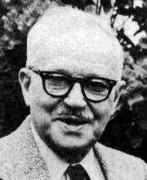
\includegraphics[height=0.2\textwidth]{static_images/neyman.jpg}
    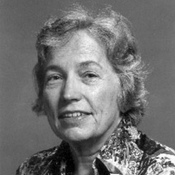
\includegraphics[height=0.2\textwidth]{static_images/ElizabethScott.jpg}
\end{figure}

...or why don't we always use the maximum likelihood estimator?

\hrulefill

Here's a toy model.  For some unknown $z_n$ and $\theta$, draw

\begin{align*}
    y_{na} | z_n, \theta \sim{}& \mathcal{N}(z_n, \theta)\\
    y_{nb} | z_n, \theta \sim{}& \mathcal{N}(z_n, \theta)
\end{align*}


\begin{align*}
    \textrm{Observations: }y ={}& (y_{11}, y_{1b}, \ldots, y_{Na}, y_{Nb})\\
    \textrm{Unknown latent variables: }z ={}& (z_1, \ldots, y_N)\\
    \textrm{Unknown global parameter: }\theta \in \mathbb{R}
\end{align*}

Task: infer $\theta$.

\end{frame}


%%%%%%%%%%%%%%%%%%%%%%%%%%%%%%%%%%%%%%%%%%%%%%%%%%%%%%%%%%%%%%%%%%%%%%%
%%%%%%%%%%%%%%%%%%%%%%%%%%%%%%%%%%%%%%%%%%%%%%%%%%%%%%%%%%%%%%%%%%%%%%%
%%%%%%%%%%%%%%%%%%%%%%%%%%%%%%%%%%%%%%%%%%%%%%%%%%%%%%%%%%%%%%%%%%%%%%%

\begin{frame}{The Neyman-Scott ``paradox''}

\begin{align*}
    y_{na} | z_n, \theta \sim{} \mathcal{N}(z_n, \theta) \quad\quad\quad
    y_{nb} | z_n, \theta \sim{} \mathcal{N}(z_n, \theta)
\end{align*}

Let's use that old workhorse, the maximum likelihood estimator (MLE)!

(\textbf{Spoiler:} Something will go wrong.)

The normal distribution gives (up to constants):

%
\begin{align*}
%
\log p(y_{na}, y_{nb} | \theta, z_n) ={}&
-\frac{1}{2} \theta^{-1} \left( y_{na}  - z_n\right)^2 - \frac{1}{2}log \theta
&-\frac{1}{2} \theta^{-1} \left( y_{nb}  - z_n\right)^2 - \frac{1}{2}\log \theta
%
\end{align*}
%

\begin{align*}
%
\log p(y | \theta, z) ={}&
\sum_{n=1}^N \log p(y_{na}, y_{nb} | \theta, z_n)
%
\end{align*}
%

The MLE is given by:

%
\begin{align*}
%
\hat\theta, \hat{z} :={}& \argmax_{\theta, z}  \log p(y | \theta, z)
\quad\quad\Leftrightarrow{}\quad\quad
\fracat{\partial \log p(y | \theta, z)}{\partial (\theta, z)}{\thetahat, \hat{z}} ={} 0
%
\end{align*}
%

\textbf{Exercise:} Find an expression for $\hat{z}_n$.

\end{frame}




%%%%%%%%%%%%%%%%%%%%%%%%%%%%%%%%%%%%%%%%%%%%%%%%%%%%%%%%%%%%%%%%%%%%%%%
%%%%%%%%%%%%%%%%%%%%%%%%%%%%%%%%%%%%%%%%%%%%%%%%%%%%%%%%%%%%%%%%%%%%%%%
%%%%%%%%%%%%%%%%%%%%%%%%%%%%%%%%%%%%%%%%%%%%%%%%%%%%%%%%%%%%%%%%%%%%%%%

\begin{frame}{The Neyman-Scott ``paradox''}

\textbf{Exercise:} Find an expression for $\hat{z}_n$.

\begin{align*}
%
0 ={}& \fracat{\partial \log p(y | \theta, z)}{\partial z_n}{\hat{z}, \thetahat} \\
={}& \fracat{\partial \log p(y_{na}, y_{nb} | \theta, z_n)}{\partial z_n}{\hat{z}, \thetahat}\\
={}& \frac{\partial}{\partial z_n}
\left(
-\frac{1}{2} \theta^{-1} \left( y_{na}  - z_n\right)^2 - \frac{1}{2}\log \theta
-\frac{1}{2} \theta^{-1} \left( y_{nb}  - z_n\right)^2 - \frac{1}{2}\log \theta
\right)
\Bigg|_{\hat{z}, \thetahat}\\
={}& - \thetahat^{-1} (y_{na}  - \hat{z}_n)
    - \thetahat^{-1} (y_{nb}  - \hat{z}_n) \Rightarrow \\
\hat{z}_n ={}& \frac{1}{2}(y_{na} + y_{nb}).
%
\end{align*}

Wonderful!  This is a very sensible expression, and it doesn't depend on
$\thetahat$.

\vspace{1em}
\textbf{Exercise:} Using this result, find an expression for $\thetahat$.

Hint:
%
$
%
\left( y_{na}  - \hat{z}_n\right)^2 =
\left( y_{nb}  - \hat{z}_n\right)^2 =
\frac{1}{4} \left( y_{na}  - y_{nb}\right)^2
%
$
%

\end{frame}



%%%%%%%%%%%%%%%%%%%%%%%%%%%%%%%%%%%%%%%%%%%%%%%%%%%%%%%%%%%%%%%%%%%%%%%
%%%%%%%%%%%%%%%%%%%%%%%%%%%%%%%%%%%%%%%%%%%%%%%%%%%%%%%%%%%%%%%%%%%%%%%
%%%%%%%%%%%%%%%%%%%%%%%%%%%%%%%%%%%%%%%%%%%%%%%%%%%%%%%%%%%%%%%%%%%%%%%

\begin{frame}{The Neyman-Scott ``paradox''}

\textbf{Exercise:} Find an expression for $\thetahat$.

Hint:
%
$%
\left( y_{na}  - \hat{z}_n\right)^2 =
\left( y_{nb}  - \hat{z}_n\right)^2 =
\frac{1}{4} \left( y_{na}  - y_{nb}\right)^2
%
$
%

\begin{align*}
%
0 ={}& \fracat{\partial \log p(y | \theta, z)}{\partial \theta}{\hat{z}, \thetahat} \\
={}& \frac{\partial}{\partial \theta}
\sumn
\left(
-\frac{1}{2} \theta^{-1} \left( y_{na}  - z_n\right)^2 - \frac{1}{2}\log \theta
-\frac{1}{2} \theta^{-1} \left( y_{nb}  - z_n\right)^2 - \frac{1}{2}\log \theta
\right)
\Bigg|_{\hat{z}, \thetahat}\\
={}&
\sumn
\left(
\frac{1}{2} \thetahat^{-2} \frac{1}{4} \left( y_{na}  - y_{nb}\right)^2 - \frac{1}{2}\thetahat^{-1} +
\frac{1}{2} \thetahat^{-2} \frac{1}{4} \left( y_{na}  - y_{nb}\right)^2 - \frac{1}{2}\thetahat^{-1}
\right)
\\={}&
\thetahat^{-2} \frac{1}{4} \sumn \left( y_{na}  - y_{nb}\right)^2 - N \thetahat^{-1}
\Rightarrow \\
\thetahat ={}& \frac{1}{4} \meann \left( y_{na}  - y_{nb}\right)^2.
%
\end{align*}

\textbf{Exercise:}
Suppose the true parameters are $\theta_0$ and $z_0$.

What is the behavior of $\thetahat$ for large $N$?

Hint: Use the law of large numbers.

\end{frame}



%%%%%%%%%%%%%%%%%%%%%%%%%%%%%%%%%%%%%%%%%%%%%%%%%%%%%%%%%%%%%%%%%%%%%%%
%%%%%%%%%%%%%%%%%%%%%%%%%%%%%%%%%%%%%%%%%%%%%%%%%%%%%%%%%%%%%%%%%%%%%%%
%%%%%%%%%%%%%%%%%%%%%%%%%%%%%%%%%%%%%%%%%%%%%%%%%%%%%%%%%%%%%%%%%%%%%%%

\begin{frame}{The Neyman-Scott ``paradox''}

\textbf{Exercise:}
What is the behavior of $\thetahat$ for large $N$?
By the law of large numbers,
%
\begin{columns}
%
\begin{column}{0.7\textwidth}
\begin{align*}
%
\thetahat &={} \frac{1}{4} \meann \left( y_{na}  - y_{nb}\right)^2\\
&\plim{} \frac{1}{4}
\expect{p(y | \theta_0, z_0)}{\left( y_{na}  - y_{nb}\right)^2}
\\&=
\frac{1}{4}
\expect{p(y | \theta_0, z_0)}{\left( y_{na} - z_{0n} - (y_{nb} - z_{0n})\right)^2}
\\&=
\frac{1}{4}\Bigg(
    \expect{p(y | \theta_0, z_0)}{( y_{na} - z_{0n})^2} +
    \expect{p(y | \theta_0, z_0)}{( y_{nb} - z_{0n})^2} +
    \\&\quad\quad\quad\quad
    2 \expect{p(y | \theta_0, z_0)}{( y_{na} - z_{0n})( y_{nb} - z_{0n})}
\Bigg)
\\&=
\frac{1}{4}\left(\theta_0 + \theta_0 + 0\right)
\\&= \frac{\theta_0}{2} \ne \theta_0.
%
\end{align*}
%
\end{column}
\begin{column}{0.3\textwidth}
    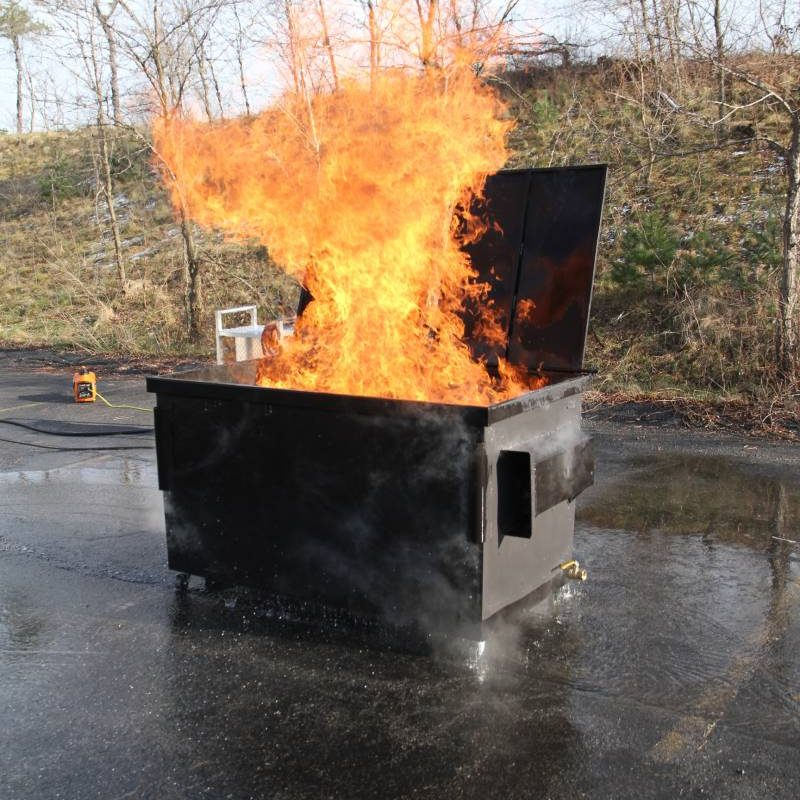
\includegraphics[width=1.0\textwidth]{static_images/dumpster.jpg}
\end{column}
\end{columns}

\vspace{2em}
$\Rightarrow$ \textbf{The MLE is inconsistent.  What went wrong?}

\end{frame}


%%%%%%%%%%%%%%%%%%%%%%%%%%%%%%%%%%%%%%%%%%%%%%%%%%%%%%%%%%%%%%%%%%%%%%%
%%%%%%%%%%%%%%%%%%%%%%%%%%%%%%%%%%%%%%%%%%%%%%%%%%%%%%%%%%%%%%%%%%%%%%%
%%%%%%%%%%%%%%%%%%%%%%%%%%%%%%%%%%%%%%%%%%%%%%%%%%%%%%%%%%%%%%%%%%%%%%%

\begin{frame}{The Neyman-Scott ``paradox''}

\textbf{The MLE is inconsistent.  What went wrong?}

\begin{align*}
\hat{z_n} &= \frac{1}{2}(y_{na} + y_{nb}) \\
\thetahat &\plim \frac{\theta_0}{2} \ne \theta_0
\end{align*}

\begin{itemize}
    %
\item Our estimates for the latent variables $\hat{z}_n$ are quite uncertain (they use only
two observaitons each)
%
\item But our MLE estimate for $\thetahat$ treated the $\hat{z}_n$ as if they
were known exactly
%
\item $\Rightarrow$ We estimated less dispersion around $\hat{z}_n$ than was
truly present.  That is, we \emph{under-estimated} $\theta_0$.
%
\item To avoid this problem, we must account for the uncertainty in $\z_n$
when estimating $\theta$.
%
\end{itemize}

Solution: \textbf{Marginalization.}

\end{frame}



%%%%%%%%%%%%%%%%%%%%%%%%%%%%%%%%%%%%%%%%%%%%%%%%%%%%%%%%%%%%%%%%%%%%%%%
%%%%%%%%%%%%%%%%%%%%%%%%%%%%%%%%%%%%%%%%%%%%%%%%%%%%%%%%%%%%%%%%%%%%%%%
%%%%%%%%%%%%%%%%%%%%%%%%%%%%%%%%%%%%%%%%%%%%%%%%%%%%%%%%%%%%%%%%%%%%%%%

\begin{frame}{Marginalization: General setup}

In general notation, we want to infer $\theta$ from
%
\begin{align*}
    \textrm{Observations: }y ={}& (y_1, \ldots, y_N)\\
    \textrm{Unknown latent variables: }z ={}& (z_1, \ldots, z_N)\\
    \textrm{Unknown global parameter: }\theta \in{}& \mathbb{R}^D
\end{align*}
%
We have learned that
%
\begin{align*}
%
\textrm{Bad: }&& \thetahat, \hat{z} ={}& \argmax_{\theta, z} \log p(y | \theta, z)\\
\textrm{Good: }&& \thetahat ={}&
    \argmax_{\theta} \log \int p(y | \theta, z) p(z | \theta) dz.
%
\end{align*}
%
\pause
%
There are two problems:
%
\begin{itemize}
    \item Need to posit $p(z | \theta)$
    \item Need to compute $\int p(y | \theta, z) p(z | \theta) dz$
\end{itemize}
%

We will only deal with the second problem in these two talks, assuming
we have a $p(z | \theta)$ we are willing to live with.

\textbf{In general, the integral is hard!}


\end{frame}



%%%%%%%%%%%%%%%%%%%%%%%%%%%%%%%%%%%%%%%%%%%%%%%%%%%%%%%%%%%%%%%%%%%%%%%
%%%%%%%%%%%%%%%%%%%%%%%%%%%%%%%%%%%%%%%%%%%%%%%%%%%%%%%%%%%%%%%%%%%%%%%
%%%%%%%%%%%%%%%%%%%%%%%%%%%%%%%%%%%%%%%%%%%%%%%%%%%%%%%%%%%%%%%%%%%%%%%

\begin{frame}{Bayesian statistics has marginalization built in}
    \href{https://rgiordan.github.io/bayes/2019/08/30/bayesian_as_inverse_problem.html}{Link to optional blog post on frequentist vs Bayesian statistics}
\end{frame}

\begin{frame}{Bayesian statistics has marginalization built in}

% \begin{align*}
%     \textrm{Observations: }y ={}& (y_1, \ldots, y_N)\\
%     \textrm{Unknown latent variables: }z ={}& (z_1, \ldots, z_N)\\
%     \textrm{Unknown global parameter: }\theta \in{}& \mathbb{R}^D \\
%     \textrm{Need to compute: } \int &p(y | \theta, z) p(z | \theta) dz
% \end{align*}

Recall that a Bayesian model posits a full generative process:
%
\begin{align*}
%
\theta \sim{} p(\theta) \quad\quad
z | \theta \sim{} p(z | \theta) \quad\quad
y | z, \theta \sim{} p(y | z, \theta)
%
\end{align*}
%
and forms the posterior
%
\begin{align*}
%
p(\theta, z \vert y) ={}& \frac{p(y | \theta, z) p(z | \theta) p(\theta)}
     {\int \int p(y | \theta', z') p(z' | \theta') p(\theta') d\theta' dz'}
 \end{align*}
%
\pause
%
\begin{align*}
\Rightarrow
 p(\theta \vert y) = \int p(\theta, z \vert y) dz
 ={}& \frac{\int p(y | \theta, z) p(z | \theta) p(\theta) \, dz}
      {\int\int p(y | \theta', z') p(z' | \theta') p(\theta') d\theta' dz'} \\
={}& \frac{\left(\int p(y | \theta, z) p(z | \theta)dz \right) p(\theta) }
   {\int\left( \int p(y | \theta', z') p(z' | \theta')dz'\right) p(\theta') d\theta' } \\
={}& \frac{ p(y | \theta) p(\theta) }
  { \int p(y | \theta') p(\theta') d\theta'}.
%
\end{align*}
%
% Inference using the ordinary posterior is the same as doing inference with
% the marginalized likelihood.
\pause
$\Rightarrow$
\textbf{Bayesian methods do not suffer from the Neyman-Scott problem.}

\begin{itemize}
    \item Bayesians are forced to posit $p(z | \theta)$
    \item Forming the posterior is equivalent to using the marginal $p(y | \theta)$
\end{itemize}

\pause
\textbf{But the integral is still hard!}
%
Full Bayesian solutions typically require Markov Chain Monte Carlo, which is
slow and sampling based.

Are there faster alternatives, based on optimization?  \textbf{Hint: Yes.}

\end{frame}



%%%%%%%%%%%%%%%%%%%%%%%%%%%%%%%%%%%%%%%%%%%%%%%%%%%%%%%%%%%%%%%%%%%%%%%
%%%%%%%%%%%%%%%%%%%%%%%%%%%%%%%%%%%%%%%%%%%%%%%%%%%%%%%%%%%%%%%%%%%%%%%
%%%%%%%%%%%%%%%%%%%%%%%%%%%%%%%%%%%%%%%%%%%%%%%%%%%%%%%%%%%%%%%%%%%%%%%

\begin{frame}{Marginalization: The EM algorithm}

One ``frequentist'' method for optimizing the marginal likelihood is the
famous expectation-maximization (EM) algorithm.

The EM algorithm works / is useful when:

\begin{itemize}
    %
    \item The joint log probability $\log p(y | \theta, z) + \log p(z | \theta)$ is easy to write down
    \item The posterior $p(z | y, \theta)$ is easy to compute
    \item The marginalizing integral $p(y | \theta) = \int p(y | \theta, z) p(z | \theta) dz$ is hard
    %
\end{itemize}

\pause
\hrulefill

The EM algorithm alternates between two steps.  Starting at an iterate
$\hat\theta_{(i)}$, repeat until convergence:

\textbf{The E-step:}  Compute $Q_{(i)}(\theta) := \expect{p\left(z | y, \hat\theta_{(i)} \right)}{\log p(y | \theta, z) + \log p(z | \theta)}$

\textbf{The M-step:}  Compute the next iterate $\thetahat_{(i + 1)} := \argmax_\theta Q_{(i)}(\theta)$

\pause
\hrulefill

Note that everything in the E- and M-steps are ``easy.''  Nevertheless, the
iterates $\thetahat_{(i)}$ converge to a (possibly local) optimum of the
marginal log likelihood $\log p(y | \theta)$.

\vspace{1em}

\pause

\textbf{Exercise: }  Prove that the EM algorithm gives a consistent estimator
for the Neyman-Scott paradox.

\end{frame}


%%%%%%%%%%%%%%%%%%%%%%%%%%%%%%%%%%%%%%%%%%%%%%%%%%%%%%%%%%%%%%%%%%%%%%%
%%%%%%%%%%%%%%%%%%%%%%%%%%%%%%%%%%%%%%%%%%%%%%%%%%%%%%%%%%%%%%%%%%%%%%%
%%%%%%%%%%%%%%%%%%%%%%%%%%%%%%%%%%%%%%%%%%%%%%%%%%%%%%%%%%%%%%%%%%%%%%%

\begin{frame}{Next week: Actual variational inference}

Next week we will:

\begin{itemize}
    %
    \item Prove that the EM algorithm works (in a non-standard way)
    \item Identify a lie I told on the last slide
    \item Generalize to cases when the posterior
        $p(z | y, \theta)$ is difficult to compute
    %
\end{itemize}

This last point will finally bring us to the set of techniques commonly called
``variational inference.''

\end{frame}


\begin{frame}{Conclusions}

\footnotesize

\bibliographystyle{plainnat}
% Hide the references header
% https://tex.stackexchange.com/questions/22645/hiding-the-title-of-the-bibliography/370784
\begingroup
\renewcommand{\section}[2]{}%
\bibliography{references}
\endgroup

\end{frame}


\end{document}
